\documentclass[a4paper,twoside,11pt]{article}
\usepackage[utf8]{inputenc}
\usepackage[english]{babel}
\usepackage{graphicx}
\usepackage{url}
\usepackage{hyperref}
\usepackage{adjustbox}

% pdflatex

% redefinição das margens das páginas
\setlength{\textheight}{24.00cm}
\setlength{\textwidth}{15.50cm}
\setlength{\topmargin}{0.35cm}
\setlength{\headheight}{0cm}
\setlength{\headsep}{0cm}
\setlength{\oddsidemargin}{0.25cm}
\setlength{\evensidemargin}{0.25cm}

\begin{document}

\begin{titlepage}
\begin{center}

% Logo
\resizebox{80mm}{!}{
\includegraphics{../img/logoISEL}}

\vspace{1cm}

% Title
{\Large \textbf{Project and Seminar}\\}
\vspace{0.3cm}
{\Large 2024/2025 - 2nd Semester\\}
\vspace{0.8cm}
{\Large Bachelor in Computer Engineering and Informatics\\}
\vspace{1cm}
{\Huge \textbf{Database Documentation}\\}
\vspace{2cm}

% Authors
\begin{tabular}{c}
    Ângelo Azevedo, n.º 50565, e-mail: \href{mailto:a50565@alunos.isel.pt}{a50565@alunos.isel.pt}\\
    António Alves, n.º 50539, e-mail: \href{mailto:a50539@alunos.isel.pt}{a50539@alunos.isel.pt}\\
\end{tabular}

\vspace{2cm}

% Supervisors
\begin{tabular}{ll}
    {Advisor:} & Pedro Matutino, e-mail: \href{mailto:pedro.miguens@isel.pt}{pedro.miguens@isel.pt} \\
    %  & Alberto Caeiro, e-mail: ac@pc.com, PersonCompany\\
\end{tabular}

\vspace{1cm}

March 2025

\end{center}
\end{titlepage}

\section*{Introduction}
This document provides a overview of the database, entities and attributes and relationships. 
It also includes implementation decisions.

\section*{Database overview}
The database has been modeled using an Entity-Relationship (ER) approach.
This approach allows for a better understading of the relationships between entities. The following section shows a figure with the ER model.

The database is implemented with PostgreSQL and tested using fake information in a postgres docker container.

The following section will address the ER model.
\section*{Entity-Relationship Model}
\begin{figure}[htbp]
	\centering
	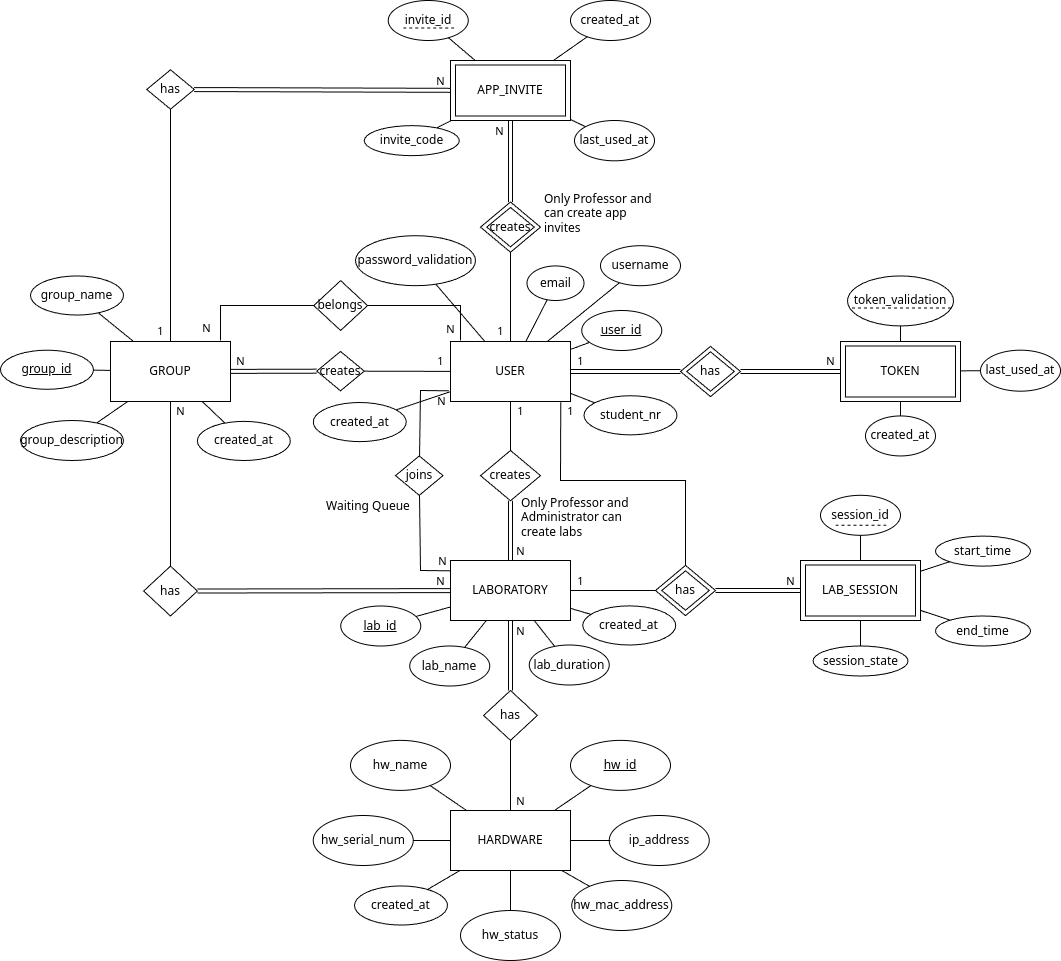
\includegraphics[width=\textwidth]{../img/ERDiagramRL.drawio}
	\caption{Entity-Relationship Model}
	\label{fig:ERModel}
\end{figure}

\section*{Entities and Attributes}
This section provides a comprehensive description of each entity and their attributes.
\subsection*{User}
The first important entity is the \textbf{User}. This entity represents a user in the database.

It has a \textbf{user\_id} as primary key and identity column. An identity column is a special column that is generated automatically from an implicit sequence.
So, whenever a user is inserted in the database it will generate a id. The user\_id is a int data type. 

It also has, as char sequence, \textbf{username}, \textbf{email} and \textbf{password\_validation}. All of them are not null and email is unique. Password\_validation is the hash of the user's password.

Finally has a \textbf{student\_nr} (student number) as Int type and unique and \textbf{created\_at} as a timestamp type and not null.
The student number can be null. This allows users, like professor or other, to be a user entity in the DB. Is worth mentioning that there is not a descriminator attribute because 
this descrimination will be implemented in the RBAC system.

\subsection*{Token}
\textbf{Token} is a weak entity because it cannot be uniquely identified by its attributes alone. This means that a token needs a user\_id to be identified. This way, token requires the user to exist.

Since it is a weak entity, it must have a partial key. This partial key is \textbf{token\_validation}. Token\_validation is a randomly generated hash. It is a char sequence and not null.

The last attributes are \textbf{created\_at} and \textbf{last\_used\_at}. Both are timestamp types and not null. 

\subsection*{App Invite}
\textbf{App Invite} is a weak entity. For the same reason as the token, this entity requires the user to exist and cannot be uniquely identified. For example an app invite should not exist if the user is deleted.

As partial key, the \textbf{invite\_id} with user\_id uniquely identify an app invite. This invite\_id is generated always as identity and is a int type.

It has an \textbf{invite\_code} attribute as char sequence and not null. This invite code can take up to 255 bytes but, the true dimension is decided by the domain.

It also has a \textbf{created\_at} and \textbf{last\_used\_at} like the token entity.

\nocite{*}
\bibliographystyle{plain}
\bibliography{references}

\end{document}